\documentclass[12pt]{article}

\usepackage[left=0.9in,right=0.9in,top=0.8in,bottom=1.05in]{geometry}
\newcommand{\ligne}[1]{\rule[0.5ex]{\textwidth}{#1}\\}

\usepackage[]{graphicx}
\usepackage{wrapfig}
\usepackage{physics}
\usepackage{color}
\usepackage{amsthm}

\definecolor{coloradoRed}{rgb}{0.80,0.27,0.16}

\usepackage[breakable]{tcolorbox}
\usepackage{graphicx}
\usepackage{enumitem}

\NewDocumentEnvironment{solution}{O{} O{no}}
{
    \begin{tcolorbox}[
        breakable,
        colback=white,
        colframe=black,
        boxrule=0.5pt,
        arc=0pt,
    ]

    \textcolor{coloradoRed}{\textbf{Result:}}\par\noindent

    \ifstrequal{#2}{yes}{
        \begin{enumerate}[label=(\alph*)]
            \item 
            \mbox{}\par
    }{}

    \if\relax\detokenize{#1}\relax
        % No image argument -- do nothing
    \else
        
            \centering
            \includegraphics[width=1.0\linewidth]{#1}
       
    \fi

    \ifstrequal{#2}{yes}{
        \end{enumerate}
    }{}
}
{
    \end{tcolorbox}
}
% \newenvironment{proof}
% {\par\noindent\textit{Proof.}}
% {\hfill\qed\par}

\begin{document}

\begin{flushleft}
    \textbf{Department of Applied Mathematics and Statistics} \\
    \textbf{COLORADO SCHOOL OF MINES} \\
    Math $550$: Numerical Solutions of Partial Differential Equations \\
    Charles Girard

\end{flushleft}


\begin{center}
\bf{Numerical PDEs Homework \#2}\\
\bf{Due Monday, November 2, 2026}
\end{center}

\vspace{0.3cm}

\noindent \textbf{Problem 1: Poisson Equation.}
Make sure the code from HW0 still works; use a finite dfference method to solve
$ \nabla^2 u = f(x,y)$ in the domain $x \in [0,2\pi], \, y \in [0,2\pi]$ with Dirichelet boundary conditions
on all sides.
Choose $f$ and boundary data so that the test solution
$$
u(x,y) = \cos(2x)\sin(2y)
$$
solves the problem. Then verify the solution converges in the second order.

\begin{solution}
    Solving for $f$ gives 
    $$
    f(x,y) = -8\cos(2x)\sin(2y).
    $$
    Using our code from HW0:
    \begin{center}
    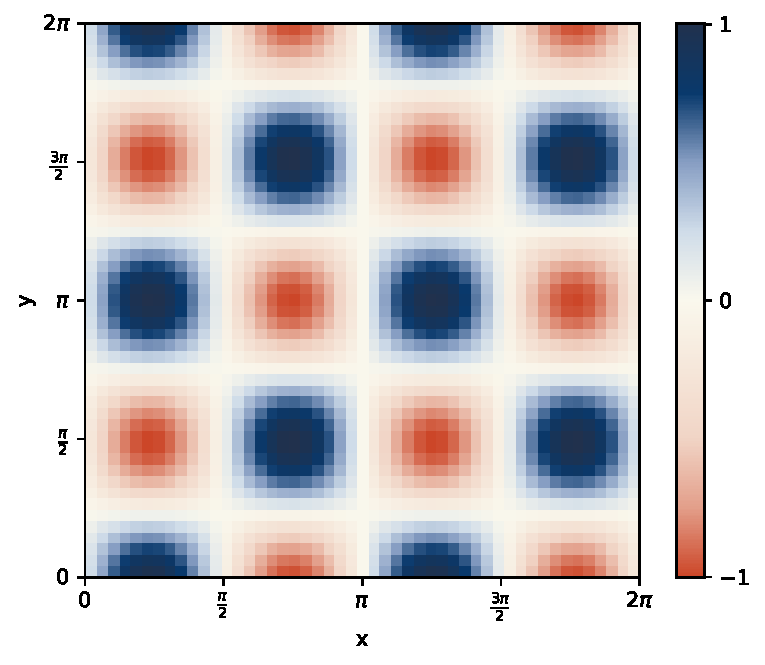
\includegraphics[width=0.7\linewidth]{u_approx.pdf}
    \par
    \small Approximate solution $u_{\text{apx}}$, with grid resolution $N=50$.
    \label{fig: HW0_approx}
    \end{center}

    \begin{center}
    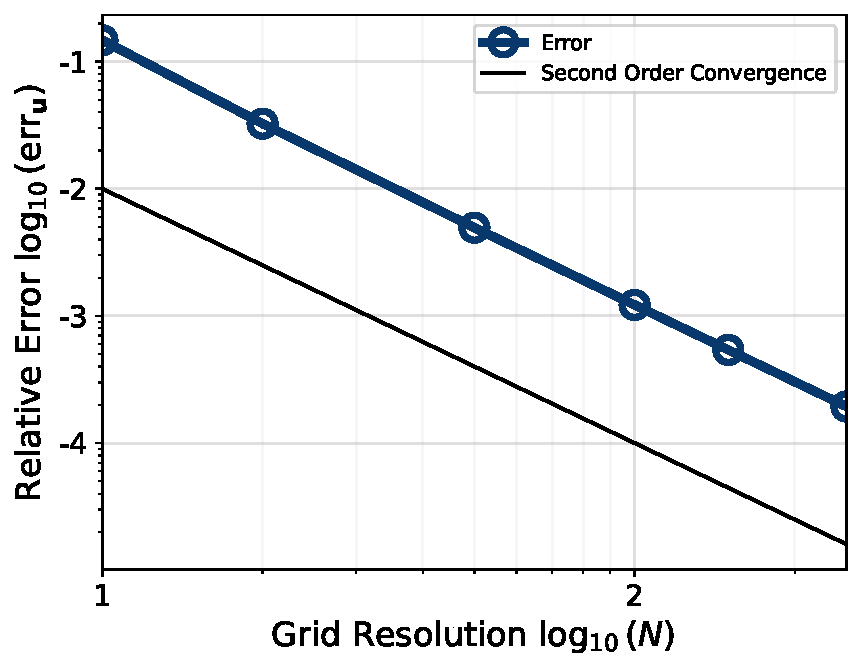
\includegraphics[width=0.7\linewidth]{HW0_Dirichilet_Convergence.pdf}
    \par
    \small Convergence plot for the Dirichlet problem.
    \end{center}
\end{solution}

\vspace{1cm}

\noindent \textbf{Problem 2: Poisson Equation with an Immersed Boundary}

Noe we'll consider an additional Dirichelet condition:
\begin{align}
u(x^{ib}, y^{ib}) = \cos(2x^{ib})\sin(2y^{ib}), \label{eq:ib_condition} \\
x^{ib} = \pi + \cos\theta, \quad y^{ib} = \pi + \sin\theta, \quad \theta \in [0, 2\pi]. \label{eq:ib_param}
\end{align}

\begin{enumerate}
\item Discretize $\left(x^{ib},y^{ib}\right)$ to have roughly the same immersed boundary resolution (point spacing) as the finite difference grid.
\item Create the spreading operator that maps the immersed boundary forces onto the finite difference grid:
    \begin{align}
    \mathcal{S}^{ib}(q) = \sum_{k=1}^{N_{ib}}q_k \delta(x - x^{ib}_k, y - y^{ib}_k) \label{eq:spreading_operator}
    \end{align},
    where $q_k$ are the forces exerted by the immersed boundary points, and
    $\delta_a$ is the 2D Gaussian with a variance $a = 1.2 \Delta x$.
\item Discretizing our new PDE, we'll have $N_{ib}$ more unknowns than equations. Therefore, we impose the dirichelet boundary condition:
    \begin{align}
        \int \int_{(x,y)} u(x,y) \delta_a(x - x^{ib}_k, y - y^{ib}_k) \, dx \, dy = u(x^{ib}_k, y^{ib}_k), \quad k = 1, \dots, N_{ib},
    \end{align}
    approximated by a discrete sum:
    \begin{align}
        \sum_{i,j} u_{i,j} \delta_a(x_i - x^{ib}_k, y_j - y^{ib}_k) \Delta x^2 = u(x^{ib}_k, y^{ib}_k), \quad k = 1, \dots, N_{ib}.
    \end{align}
    Call the operator on $u$ as $\mathcal{J}^{ib}(u)$.
\begin{solution}
After creasing $\mathcal{S}^{ib}$ and $\mathcal{J}^{ib}$, we ensure that it interpolates the solution at the immersed boundary points correctly:
    \begin{center}
    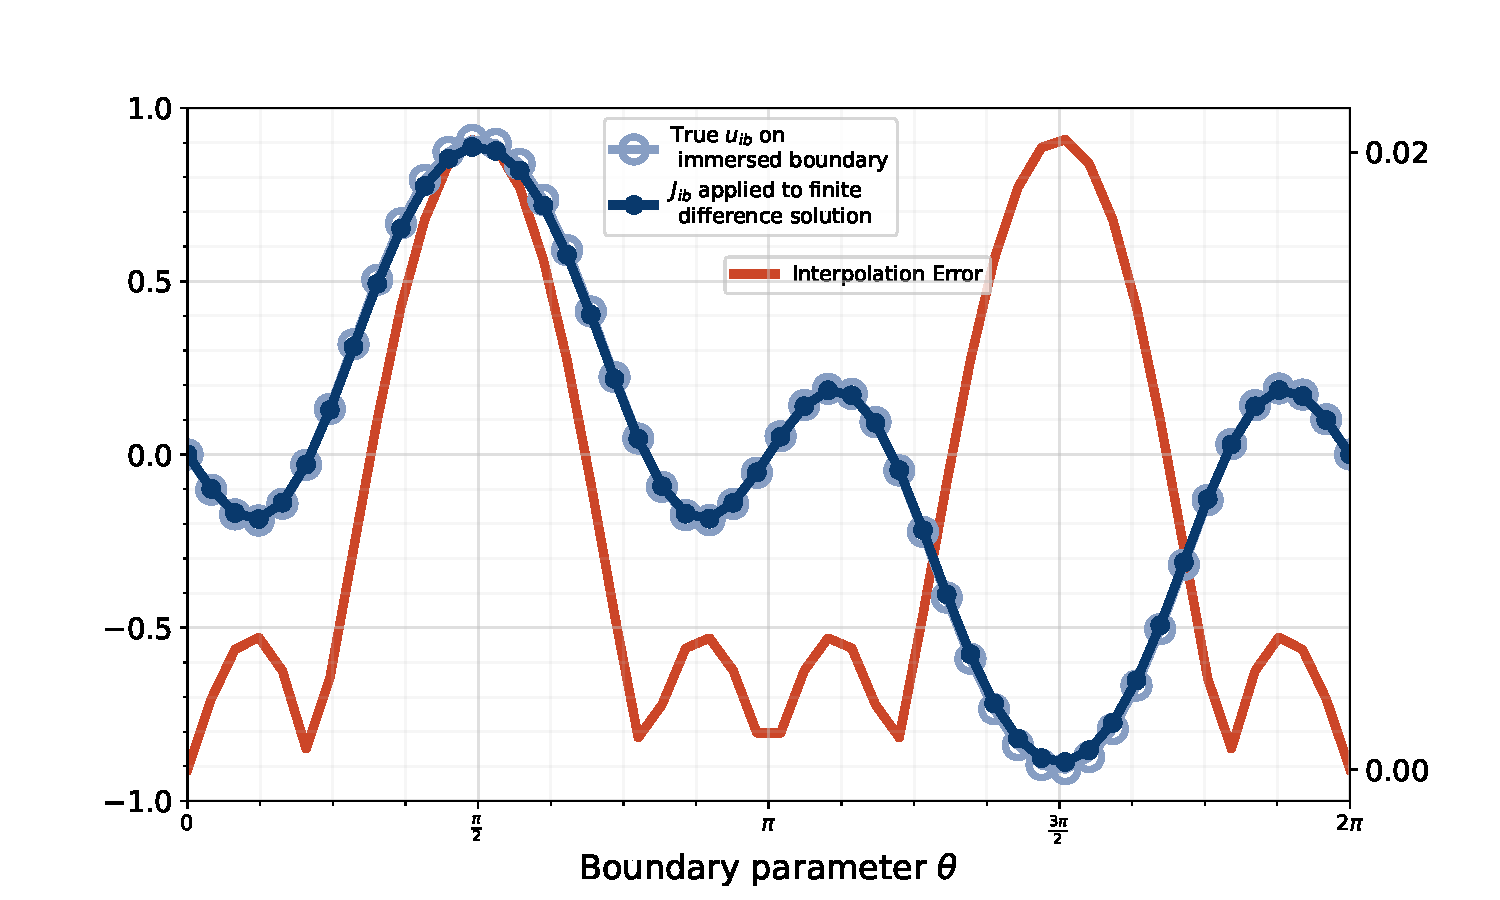
\includegraphics[width=0.7\linewidth]{interpolation_error_plot.pdf}
    \par
    \small Interpolation error at the immersed boundary points.
    \end{center}
    Note that $\left(\mathcal{J}^{ib}\right)\top = \mathcal{S}^{ib}$. Therefore, we can use this relationship to instill confidence in $\mathcal{S}^{ib}$ given we're satisfied with $\mathcal{J}^{ib}$.
\end{solution}
\item Discretize and solve the saddle point system,
\begin{align}
    \begin{bmatrix}
        \nabla^2 & -\mathcal{S}^{ib} \\
        \mathcal{J}^{ib} & 0
    \end{bmatrix}
    \begin{bmatrix}
    u(x,y) \\ q
    \end{bmatrix}
    = \begin{bmatrix}
    f(x,y) - \nabla_\text{bdy}^2 u(x,y)\\ 
    u(x^{ib}_k, y^{ib}_k)
    \end{bmatrix}
\end{align}

\begin{solution}
\begin{center}
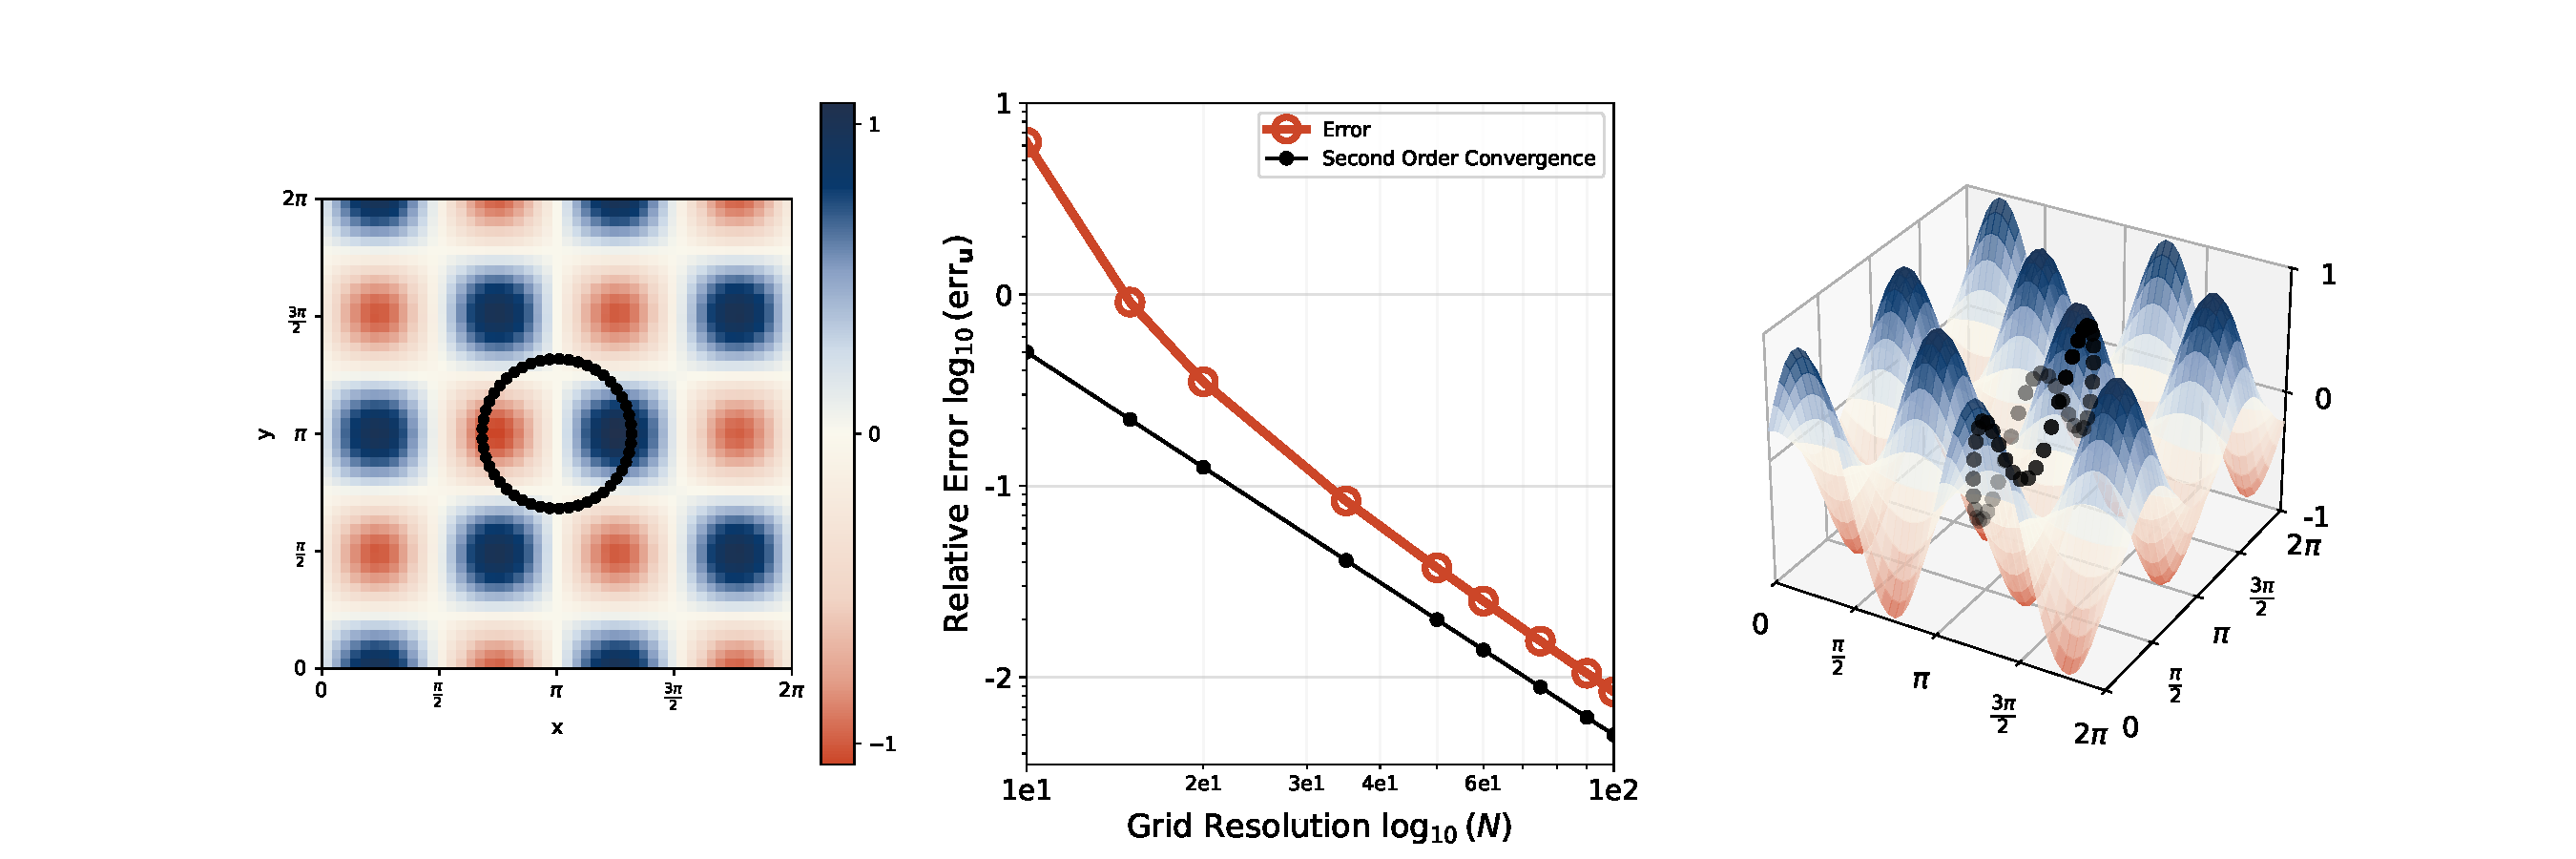
\includegraphics[width=0.95\linewidth]{HW2_ib_complete_1.pdf}
\par
\small Complete solution with the immersed boundary.
\end{center}
\end{solution}

\end{enumerate}

\vspace{1cm}
\noindent \textbf{Problem 3: An almost minimal surface}
Not to solve a problem we don't know the answer to:
\begin{align}
\nabla^2 u = \mathcal{S}^{ib}(q), \\
u(0, y) = u(2 \pi, y) = u(x, 0) = u(x, 2 \pi) = 0, \\
u(x^{ib}_k, y^{ib}_k) = \cos(2x^{ib})\sin(2y^{ib}), 
x^{ib} = \pi + \cos\theta, \quad y^{ib} = \pi + \sin\theta, \quad \theta \in [0, 2\pi].
\end{align}
\begin{solution}
\begin{center}
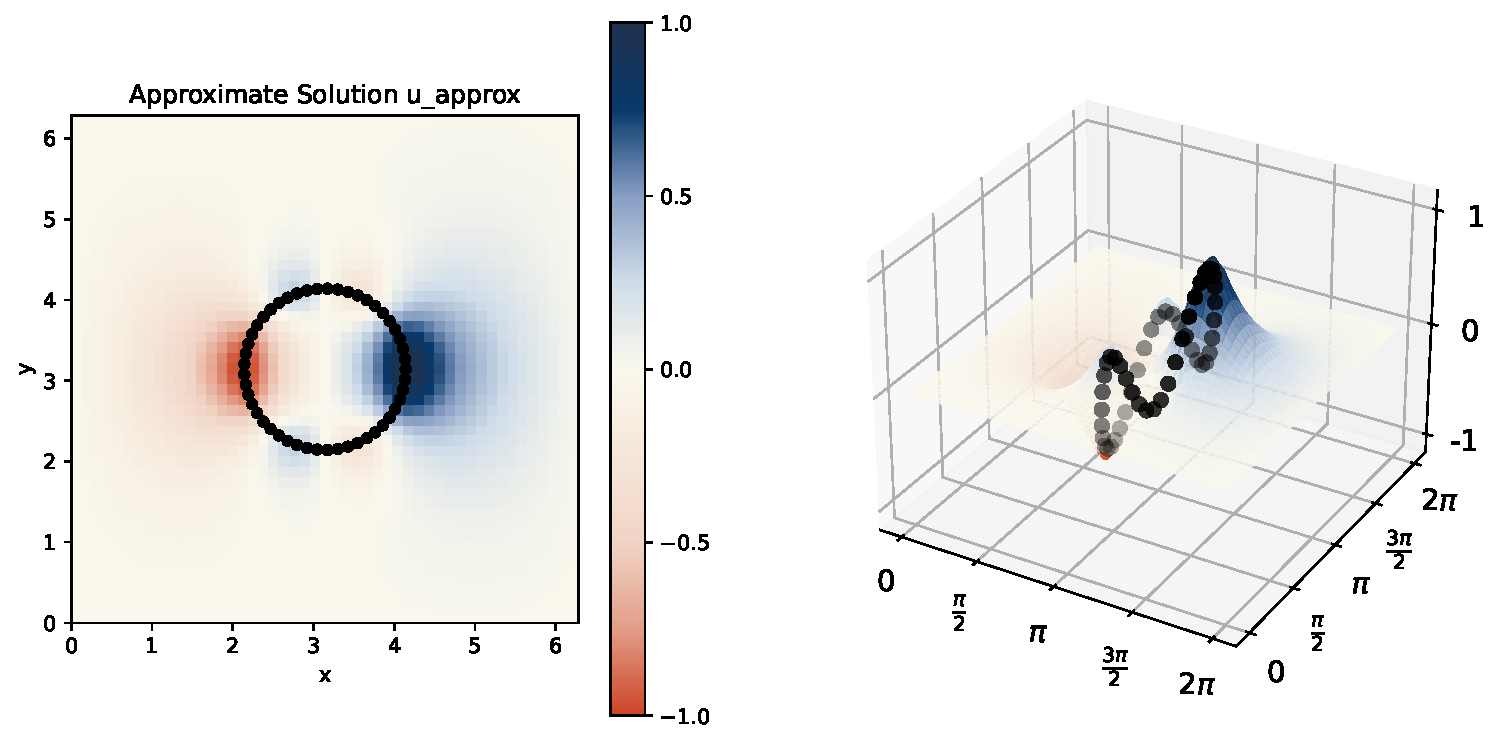
\includegraphics[width=0.95\linewidth]{u_minimal_surface.pdf}
\par
\small Approximate solution for the almost minimal surface problem.
\end{center}
\end{solution}

\vspace{1cm}
\noindent \textbf{Problem 4: Charlie's Rule}
Play around with your cool code.

\begin{solution}

The reason this submission is so close to the very generous extended deadline is due to the
over-ambitious tendencies of the author. That being said, 
please see the file in the repository titled \texttt{immersed\_boundary.gif}

No further explanation or figures are provided here, so as not to spoil the surprise.

Hopefully it doesn't disappoint.

-CG

(PS I was able to make it work more quickly with Schur decomposition! Thankfully the immersed boundary locations are unchanging, so the 
most time consuming part of making $\mathcal{S}^{ib}$ and $\mathcal{J}^{ib}$ is done only once.)

\end{solution}

\end{document}